\documentclass{article}

\usepackage{amsmath,amssymb,fullpage,graphicx}

\begin{document}

\begin{flushright}
Mikola Lysenko \\
CS704 \\
Problem Set 3
\end{flushright}


\paragraph{2.a}
Here is a version written in C++:

\begin{verbatim}
void DotProduct_gen(vector<int> x)
{
    printf("int DotProduct_sp(vector<int> y) { return ");	
    if(x.size() == 0)
        printf("0");
    for(int i=0; i<x.size(); i++)
    {
        if(i > 0)
            printf("+");
        printf("%d*y[%d]", x[i], i); 
    }
    printf("; }");
}
\end{verbatim}

\paragraph{2.b}

Based on the principle that we are given more information sooner, it ought to be possible to apply greater human insight and domain specific knowledge to the optimization problem.

\paragraph{2.c}

\[ |[ cogen ]| p =_{df} |[ pe ]| [pe, pe, p]  = |[ pe ]| [pe, p] = |[pe ]| p = p-gen \]

\paragraph{3}

The time complexity for multiplying an $m \times n$ matrix by a single $n$ dimensional row-vector is $O(mn)$ (which is optimal with respect to the input entropy).  So, the complexity of the unevaluated algorithm is $O(mn + np)$, which when applied to $k$ vectors gives the cost:
\[ T_{uneval}(m, n, p, k) = O(k(mn + np)) \]

The time complexity of evaluating the symbolic composition depends on the precise value of, $\omega$, the matrix multiplication exponent.  It is true that for multiplying two $n \times n$ matrices, $2 \leq \omega \leq \log_2(5)$.  It is conjectured that this should carry through to the multiplication of a pair of $m \times n$, $n \times p$ matrices giving the asymptotically optimal cost of multiplication, $T(m,n,p)$ as:
\[ T(m, n, p) = O( mn + np + m n^{\omega - 2} p) \]
And so the time complexity of computing the product for $k$ vectors is:
\[ T_{symbolic}(m, n, p, k) = O( mn + np + m n^{\omega - 2} p + k m p ) \]

We now asymptotically compute the bounds on $m, n, p, k$ such that $T_{symbolic} < T_{uneval}$.  Cancelling terms, we get the asymptotic expansion:
\[ k (m n + n p - m p) > m n^{\omega - 2} p\]
The complete analysis breaks down into 2 cases:

\begin{itemize}
\item[i.] $n \in o(m + p)$: in which case it is always true that $T_{uneval} > T_{symbolic}$ (by the rearrangement inequality).

\item[ii.] $n \in \Omega(m + p)$:  Without loss of generality, assume that $m > p$ (the other case is simply a transposition of $m,p$).  Then the leading order term is $kmn$ on the left hand side, and so we must require that $k \in  \Omega( p n^{\omega - 3} )$.  Note that if $\omega = 2$, then this is true for all values of $k$.
\end{itemize}

\paragraph{4.a}
\begin{center}
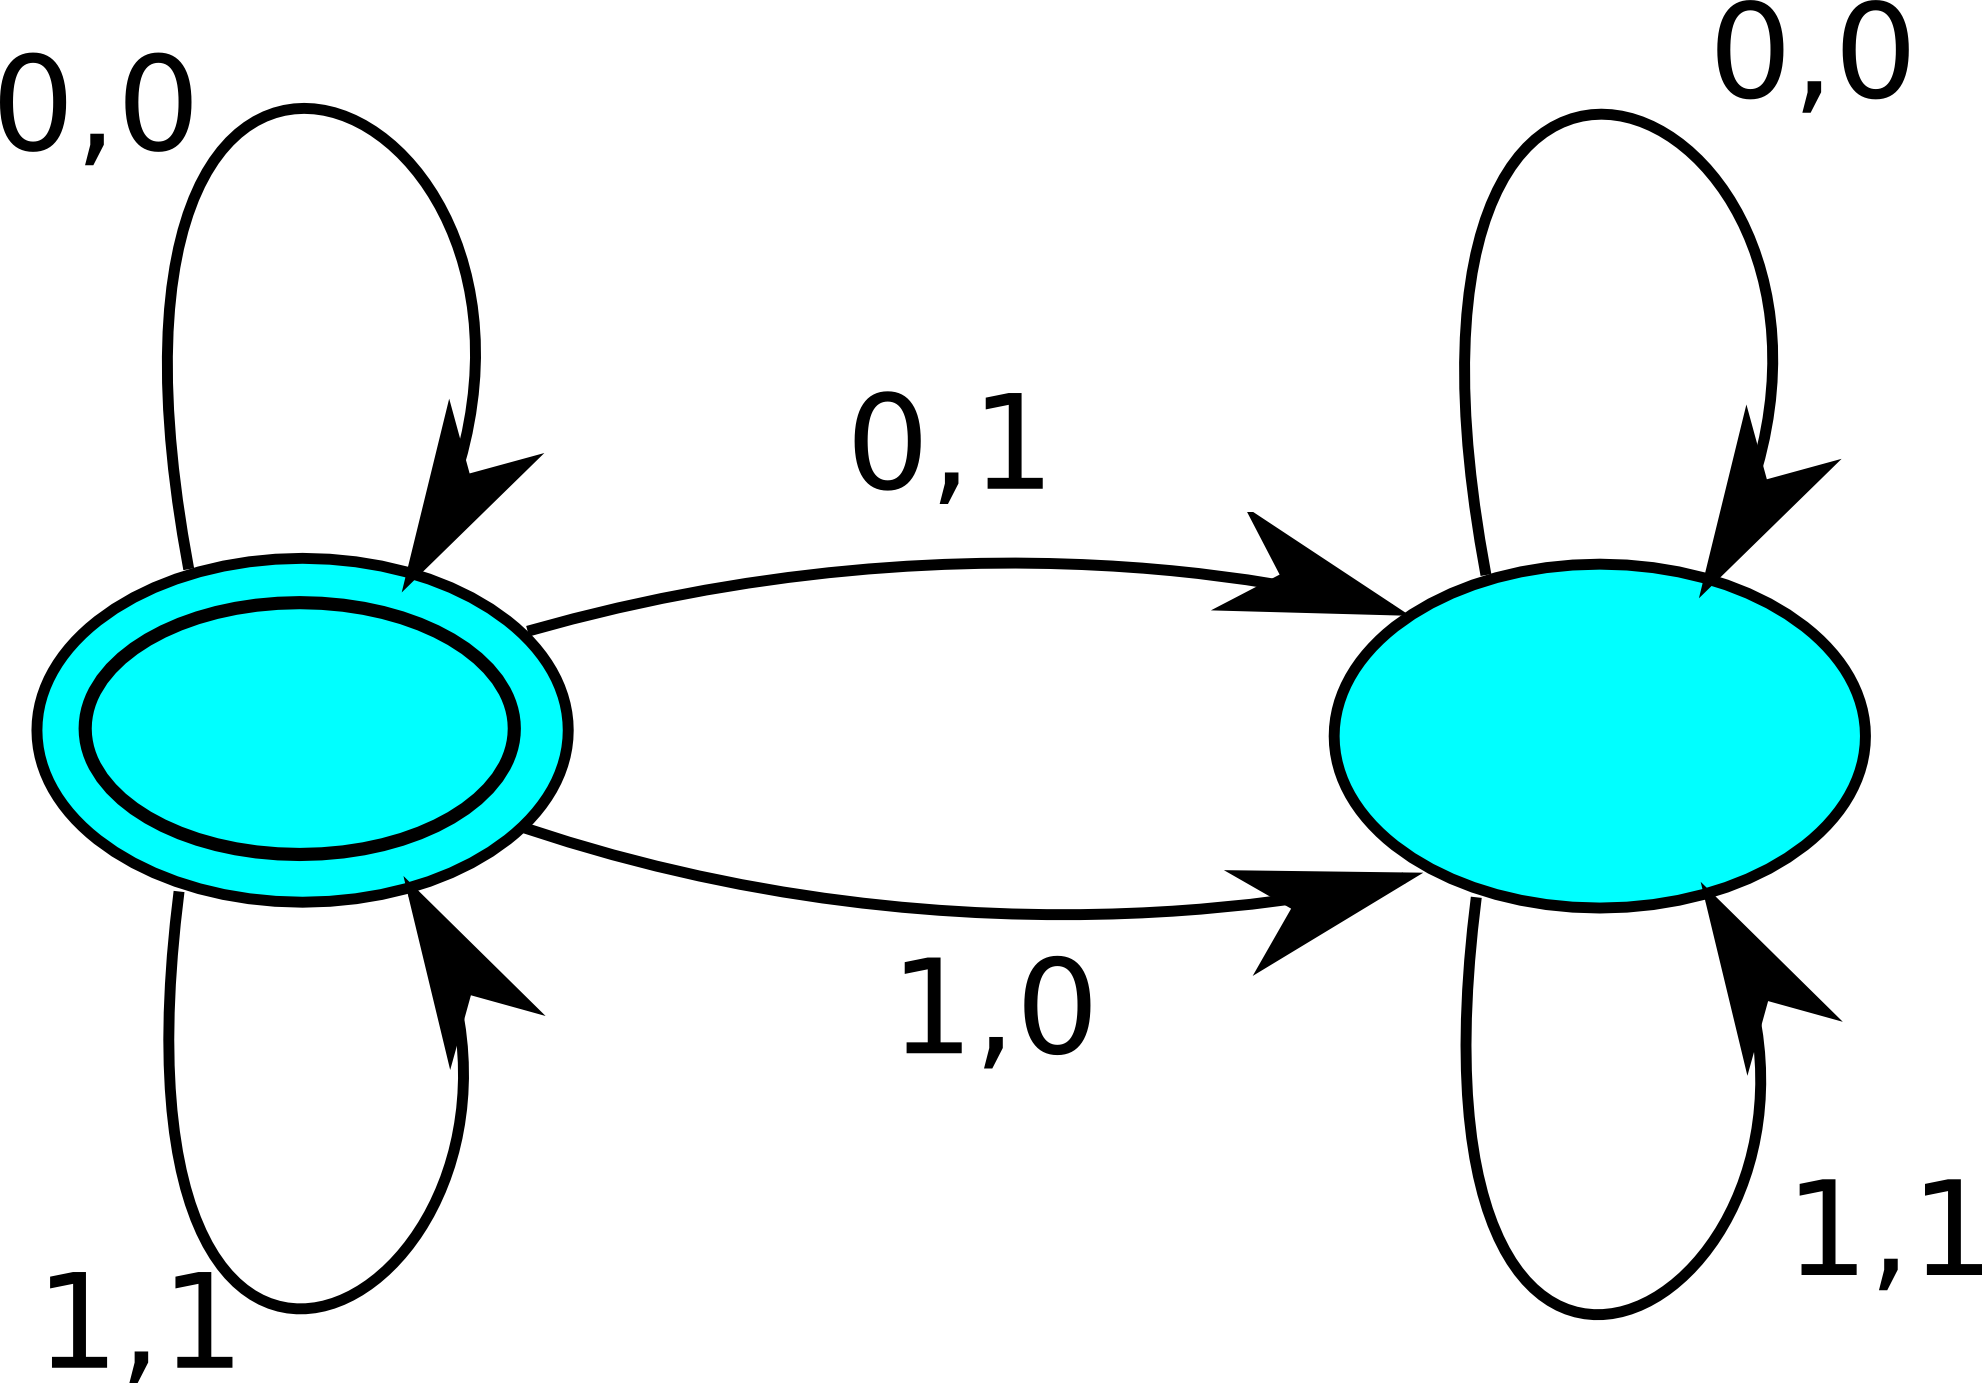
\includegraphics[height=1.5in]{ndta.png}
\end{center}

\paragraph{4.b}
Given a pair of nondeterministic transducers $M = ( Q^M, \Sigma, \Delta, \lambda^M, q^M_0), N = (Q^N, \Delta, \Gamma, \lambda^N, q^N_0)$; we give a na\
ive construction to obtain a new transduver $P = (Q^P, \Sigma, \Gamma, \lambda^P, q^P_0)$ which is the composition of $M, N$.  To do this, pick:
\begin{eqnarray*}
Q^P & = & Q^M \otimes Q^N \\
q^P_0 & = & q^M_0 \otimes q^N_0 \\
\lambda^P & = & \{ (s_0 \otimes t_0, \sigma, \gamma, s_1 \otimes t_1)) | 
(s_0, \sigma, \delta, s_1) \in \lambda^M, 
(t_0, \delta, \gamma, t_1) \in \lambda^N \}
\end{eqnarray*}
To prove that $P$ is the composition of $M, N$, we show a bisimulation between the labelled transition systems $P$ and $N \circ M$.  Indeed the states in $N \circ M$ are naturally isomorphic to $Q^M \otimes Q^N = Q^P$.  Moreover, for any transition in $P$, it is obvious that there is a pair of transitions in $\lambda^M \otimes \lambda^N$ and so $P$ is properly simulated by $N \circ M$.  So, all that remains is to show that the valid transitions in $N \circ M$ are simulated in $\lambda^P$.  But, this must be the case since for all transitions $(s_0, \sigma, \delta, s_1) \in \lambda^M$, only transitions of the form $(t_0, \delta, \gamma, t_1) \in \lambda^N$ may occur; and so $\lambda^P \cong \lambda^{N \circ M}$.

\paragraph{4.c}
\begin{center}
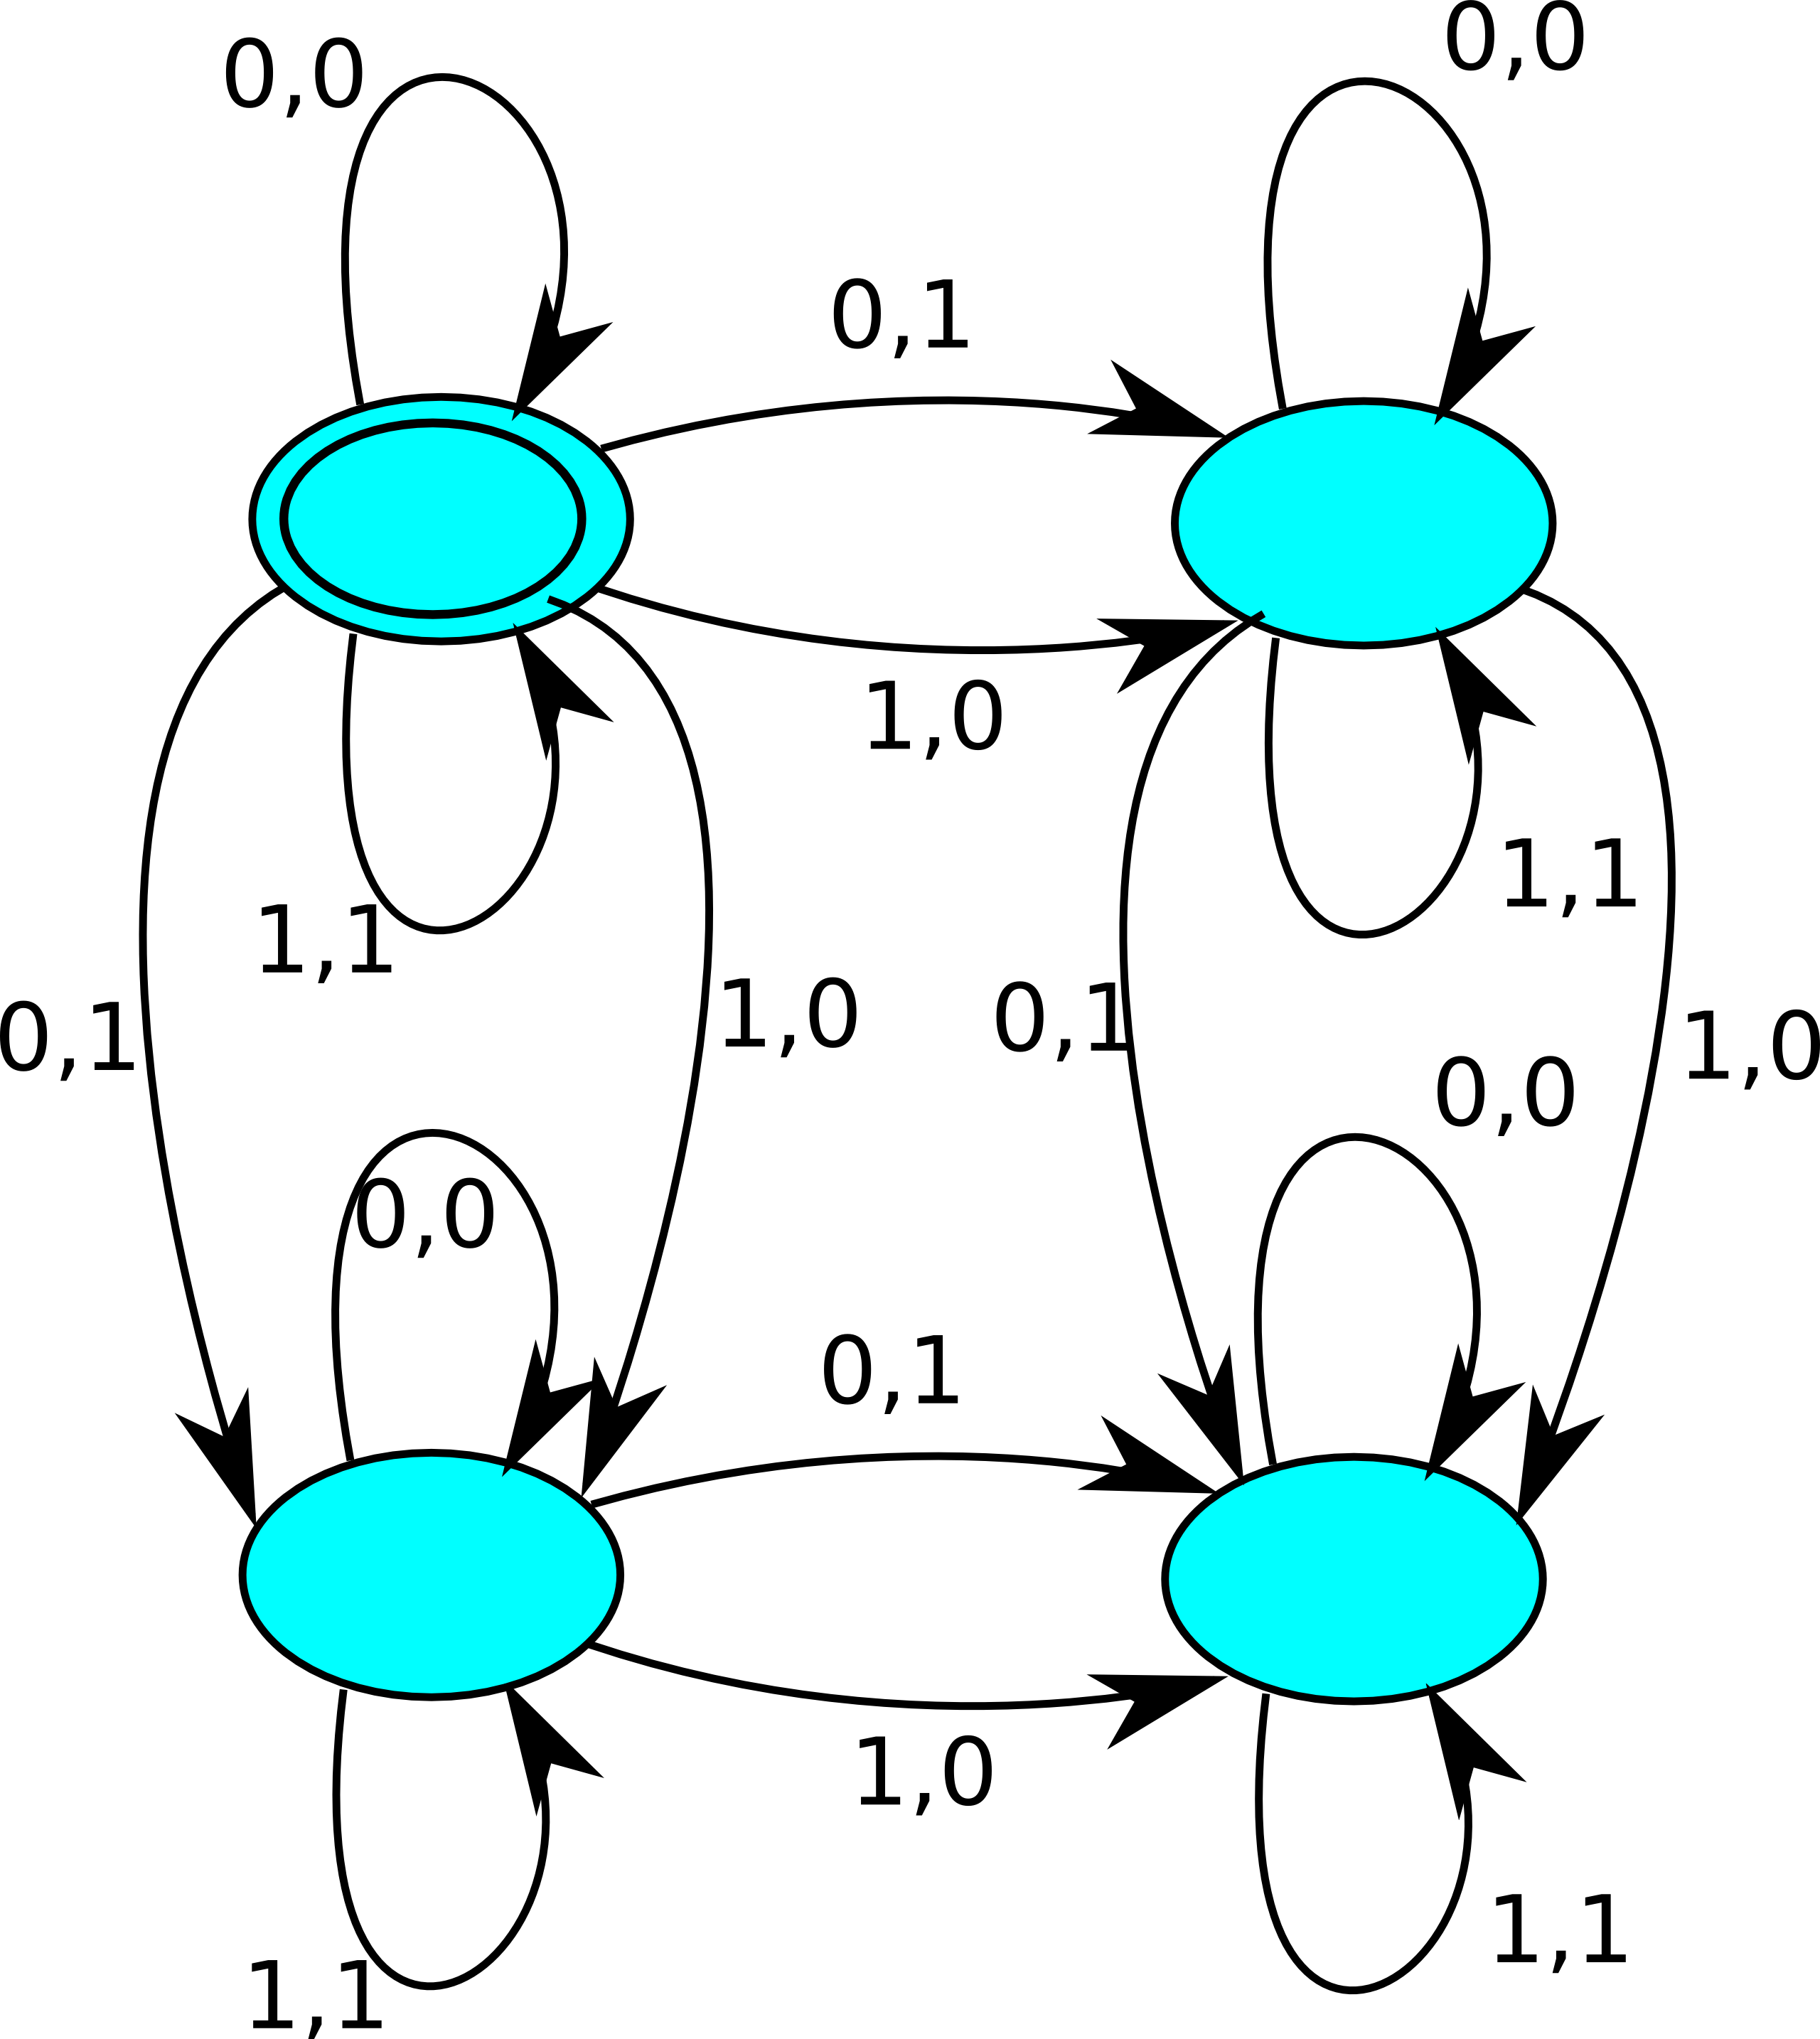
\includegraphics[height=3in]{ndta2.png}
\end{center}



\end{document}
